\documentclass[14pt, a4paper, reqno, oneside]{book}
\usepackage{amssymb,latexsym,amscd,amsmath,amsfonts,enumerate,supertabular,enumitem,fancyhdr}
\usepackage{amsmath,amsxtra,amssymb,latexsym, amscd,amsthm}

\usepackage{subfigure}
\usepackage{titlesec}
\usepackage[usehighlevels]{alnumsec}
\usepackage{indentfirst}
\usepackage[utf8]{vietnam}
%\usepackage{amsmath}
 \usepackage{graphics}
 \usepackage{graphicx}
\usepackage{tabularx}
\usepackage{epic, eepic}
\usepackage{lineno}
 \usepackage{array}
\usepackage[mathscr]{eucal}
%\usepackage{amsfonts}
\usepackage[unicode]{hyperref}
\usepackage{titledot}
\usepackage[top=3cm, bottom=3cm, left=3.5cm, right=2cm] {geometry}
\usepackage{eso-pic,calc}
\usepackage{makeidx}
\usepackage{float}
\listfiles
\titlename{Chương}
%\swapnumbers
\usepackage{listings}
\usepackage{color} % tô màu cho cod
\definecolor{dkgreen}{rgb}{0,0.6,0}
\definecolor{gray}{rgb}{0.5,0.5,0.5}
\definecolor{mauve}{rgb}{0.58,0,0.82}
\lstset{frame=tb,
	language=Python,
	aboveskip=3mm,
	belowskip=3mm,
	showstringspaces=false,
	columns=flexible,
	basicstyle={\small\ttfamily},
	numbers=none,
	numberstyle=\tiny\color{gray},
	keywordstyle=\color{blue},
	commentstyle=\color{dkgreen},
	stringstyle=\color{mauve},
	breaklines=true,
	breakatwhitespace=true,
	tabsize=3
}
\newtheorem{prof}{}
\newtheorem {theorem}{Định lý}[section]
\newtheorem {corollary}[theorem]{Hệ quả}
\newtheorem {lemma}[theorem]{Bổ đề}
\newtheorem {proposition}[theorem]{Mệnh đề}
\newtheorem {definition}[theorem]{Định nghĩa}
\newtheorem{tc}[theorem]{Tiêu chuẩn}
\newtheorem*{main}{Mệnh đề}
\theoremstyle {definition}
\newtheorem {remark}[theorem]{Chú ý}
\newtheorem {example}[theorem]{Ví dụ}
\newtheorem {notation}[theorem]{Kí hiệu}
\newtheorem {note}[theorem]{Nhận xét}
\renewcommand{\proofname}{\textbf{\textit{Chứng minh}}}
\renewcommand{\bibname}{TÀI LIỆU THAM KHẢO}
\renewcommand{\chaptername}{CHƯƠNG}
\renewcommand{\thechapter}{\arabic{chapter}}
\renewcommand{\thesection}{\thechapter.\arabic{section}}
\renewcommand{\thesubsection}{\thesection.\arabic{subsection}}
\renewcommand{\contentsname}{\hspace{100pt}MỤC LỤC}
\newenvironment{example1}[1][Ví dụ 1]{\begin{trivlist}
\item[\hskip \labelsep {\bfseries #1}]}{\end{trivlist}}
\newenvironment{example2}[1][Ví dụ 2]{\begin{trivlist}
\item[\hskip \labelsep {\bfseries #1}]}{\end{trivlist}}
\newenvironment{example3}[1][Ví dụ 3]{\begin{trivlist}
\item[\hskip \labelsep {\bfseries #1}]}{\end{trivlist}}
\newcommand{\dn}[1]{\frac{\partial #1}{\partial \nu }}

\titleformat{\section}
{\normalfont\bfseries}{\thesection.}{1em}{\fontsize 16}{}
\titleformat{\subsection}
{\normalfont\itshape}{\thesubsection.}{1em}{\fontsize 16}{}
\titleformat{\subsubsection}
{\normalfont\bfseries}{\thesubsubsection.}{1em}{\fontsize 14}{}

\def\ba{\mathbf{a}}
\def\bb{\mathbf{b}}
\def\bd{\mathbf{d}}
\def\be{\mathbf{e}}
\def\bm{\mathbf{m}}
\def\bK{\mathbf{K}}
\def\bk{\mathbf{k}}
\def\bM{\mathbf{M}}
\def\bp{\mathbf{p}}
\def\bq{\mathbf{q}}
\def\bx{\mathbf{x}}
\def\by{\mathbf{y}}
\def\bz{\mathbf{z}}
\def\bu{\mathbf{u}}
\def\bv{\mathbf{v}}
\def\bw{\mathbf{w}}

\def\bbx{\bar{\mathbf{x}}}
\def\bbX{\bar{\mathbf{X}}}
\def\bbw{\bar{\mathbf{w}}}

\def\bE{\mathbf{E}}
\def\bX{\mathbf{X}}
\def\bY{\mathbf{Y}}
\def\bZ{\mathbf{Z}}
\def\bA{\mathbf{A}}
\def\bB{\mathbf{B}}
\def\bC{\mathbf{C}}
\def\bP{\mathbf{P}}
\def\bQ{\mathbf{Q}}
\def\bI{\mathbf{W}}
\def\bS{\mathbf{S}}
\def\bT{\mathbf{T}}
\def\bW{\mathbf{W}}
\def\bI{\mathbf{I}}
\def\bL{\mathbf{L}}
\def\bU{\mathbf{U}}
\def\bzero{\mathbf{0}}
\def\bone{\mathbf{1}}
\def\R{\mathbb{R}}
\def\L{\mathcal{L}} 
\def\S{\mathcal{S}} 


\def\bmt{\left[\begin{matrix}}
	\def\bmt{\end{matrix}\right]}

\def\diag{\text{diag}}

\def\bmt{\left[\begin{matrix}}
	\def\emt{\end{matrix}\right]}

\def\blambda{\boldsymbol{\lambda}}
\def\bxi{\boldsymbol{\xi}}
\def\bSigma{\mathbf{\Sigma}}
\def\bLambda{\boldsymbol{\Lambda}}
\def\bnu{\boldsymbol{\nu}}
\def\bmu{\boldsymbol{\mu}}

% \def\dpcm{\hfill $\square$} % Điều phải chứng minh. 
\def\dpcm{} % Điều phải chứng minh. 
\def\tcr{\textcolor{red}}
\def\tcb{\textcolor{blue}}
\def\trace{\text{trace}}
\def\rank{\text{rank}}
\def\sgn{\text{sgn}}
\def\assign{\leftarrow}
\def\imply{\Rightarrow}
\def\dom{\textbf{dom}}

\def\lg{\textit{\textbf{Lời giải}}:}
\def\vd{\textbf{Ví dụ}: }
\def\kq{{{Kết quả:}}}

\def\tenchuongi{\text{Khái quát về CNN và bài toán chuẩn đoán bệnh lao.}}
\def\tenchuongii{\text{Một số mô hình hỗ trợ chuẩn đoán.}}
\def\tenchuongiii{\text{Chương trình thử nghiệm.}}
% Tự định nghĩa
\DeclareMathOperator*{\argmin}{argmin}
\DeclareMathOperator*{\argmax}{argmax}

\fancypagestyle{danh_trang_tren_header}{%
	\fancyhf{}
	\fancyhead[C]{\thepage}
	\renewcommand{\headrulewidth}{0.3pt}
}

\newcommand{\chapnum}[1]{\centering{CHƯƠNG #1}}
\makeatletter
\def\@makechapterhead#1{%
 \vspace{1.5\baselineskip}%
 {\parindent \z@ \raggedright \reset@font
 \ifnum \c@secnumdepth >\m@ne
 \Large\bfseries \chapnum{\thechapter}%
     %sửa ở đây, ví dụ LARGE --> cỡ to, bfseries -->đậm.
 \par\nobreak
 \vskip.5\baselineskip\relax
 \fi
 #1\par\nobreak
 \vskip\baselineskip
 }}
\makeatother
\setcounter{secnumdepth}{4}
\numberwithin{equation}{section}
\makeindex
\begin{document}
\large
%+============================================================================
\newpage
\pagestyle{danh_trang_tren_header}
\fontsize{14pt}{25pt}\selectfont
\pagenumbering{roman}
{
\chapter*{ \begin{center}
LỜI CAM ĐOAN
\end{center}}
\addcontentsline{toc}{chapter}{Lời cam đoan}
\indent Tôi xin cam đoan: Luận văn thạc sỹ chuyên ngành Khoa học máy tính, tên đề tài “Nghiên cứu hỗ trợ chuẩn đoán bệnh lao dựa vào học máy” là công trình nghiên cứu, tìm hiểu và trình bày do tôi thực hiện dưới sự hướng dẫn khoa học của \textbf{PGS.TS. Đỗ Năng Toàn},  Viện Công nghệ Thông tin, Viện Hàn lâm Khoa học và Công nghệ Việt Nam. 

Kết quả tìm hiểu, nghiên cứu trong luận văn là hoàn toàn trung thực, không vi phạm bất cứ điều gì trong luật sở hữu trí tuệ và pháp luật Việt Nam. Nếu sai, tôi hoàn toàn chịu trách nhiệm trước pháp luật.

Tất cả các tài liệu, bài báo, khóa luận, công cụ phần mềm của các tác giả khác được sử dụng lại trong luận văn này đều được chỉ dẫn tường minh về tác giả và đều có trong danh mục tài liệu tham khảo.


\vspace{14pt}
\begin{flushright}
\textit{Thái Nguyên, ngày 30 tháng 6 năm 2022.}\\
Học viên
\vspace{2.5cm}

\textbf{Nguyễn Hữu Khánh}
\end{flushright}
 

\chapter*{ \begin{center}
LỜI CẢM ƠN
\end{center}}
\addcontentsline{toc}{chapter}{Lời cảm ơn}
\vspace{10pt} 
Tác giả xin chân thành cảm ơn \textbf{PGS.TS. Đỗ Năng Toàn}, Viện Công nghệ Thông tin, Viện Hàn lâm Khoa học và Công nghệ Việt Nam, là giáo viên hướng dẫn khoa học đã hướng dẫn tác giả hoàn thành luận văn này, xin được cảm ơn các thầy, cô giáo trường Đại học công nghệ thông tin và truyền thông nơi tác giả theo học và hoàn thành chương trình cao học đã nhiệt tình giảng dạy và giúp đỡ. 

Xin cảm ơn Trung tâm Đào tạo Từ xa - Đại học Thái Nguyên nơi tác giả công tác đã tạo mọi điều kiện thuận lợi để tác giả có thời gian, tâm trí để hoàn thành nhiệm vụ nghiên cứu và chương trình học tập. 

Và cuối cùng xin cảm ơn gia đình, bạn bè, đồng nghiệp đã động viên, giúp đỡ tác giả trong suốt thời gian học tập, nghiên cứu và hoàn thành luận văn này.

Xin chân thành cảm ơn.

\begin{flushright}
\textit{Thái Nguyên, ngày 30 tháng 06 năm 2022}
\vspace{14pt}


Tác giả luận văn

\textbf{Nguyễn Hữu Khánh}
\end{flushright}

\addcontentsline{toc}{chapter}{Danh sách hình vẽ}
\listoffigures
%\addcontentsline{toc}{chapter}{Danh sách bảng}
%\listoftables
%\input {kyhieu}
\tableofcontents
\newpage
}
\chapter*{ \begin{center}
MỞ ĐẦU
\end{center}}
\addcontentsline{toc}{chapter}{Mở đầu}
% \centerline{\bf \large\MakeUppercase{LỜI NÓI ĐẦU}}
\vspace{10pt}
Theo báo cáo của Tổ chức Y tế thế giới (TCYTTG - WHO Report 2020 - Global Tuberculosis Control) \cite{gtcreport}, mặc dù đã đạt được một số thành tựu đáng kể trong công tác chống lao trong thời gian qua, bệnh lao vẫn đang tiếp tục là một trong các vấn đề sức khoẻ cộng đồng chính trên toàn cầu. TCYTTG ước tính năm 2019 trên toàn cầu có khoảng 10 triệu người hiện mắc lao, một con số đã giảm rất chậm trong những năm gần đây; 8,2\% trong số mắc lao có đồng nhiễm HIV. Bệnh lao là nguyên nhân gây tử vong đứng hàng thứ hai trong các bệnh nhiễm trùng với khoảng 1,2 triệu người tử vong do lao và khoảng 208.000 người chết do lao trong số những người nhiễm HIV. Số tử vong này làm cho lao là một trong các bệnh gây tử vong hàng đầu ở nữ giới. WHO đã công bố kết quả của mô hình đánh giá tác động ngắn hạn của đại dịch Covid-19 lên số ca tử vong do lao trong năm 2020. Kết quả cho thấy rằng tử vong do lao có thể tăng đáng kể trong năm 2020 và sẽ ảnh hưởng đến nhóm bệnh nhân lao dễ bị tổn thương nhất, tăng khoảng 200.000 – 400.000 ca tử vong, nếu như các dịch vụ chẩn đoán và phát hiện bệnh nhân trên toàn cầu bị ngưng trệ và giảm từ 25 – 50\% trong khoảng 3 tháng. Con số tử vong sẽ tương ứng với mức tử vong toàn cầu do lao vào năm 2015, một bước lùi nghiêm trọng trong quá trình hướng tới mục tiêu của Hội nghị Cấp Cao Liên Hợp Quốc về Lao và Chiến lược thanh toán bệnh lao của WHO.

Về Việt nam, hiện chúng ta vẫn là nước có gánh nặng bệnh lao cao, đứng thứ 11 trong 30 nước có số người bệnh lao cao nhất trên toàn cầu, đồng thời đứng thứ 11 trong số 30 nước có gánh nặng bệnh lao kháng đa thuốc cao nhất thế giới (báo cáo WHO 2020). Bệnh lao vẫn là một trong những bệnh truyền nhiễm phổ biến ở Việt Nam. Hàng năm, ước tính có 17.000 trường hợp tử vong do lao tại Việt Nam, cao hơn gấp hai lần so với con số tử vong do tai nạn giao thông. Mỗi năm ước tính có 180.000 người có bệnh lao hoạt động; 5.000 trường hợp trong số đó được xác định nhiễm lao kháng đa thuốc. Chẩn đoán bệnh lao không thật sự khó trong đa số các trường hợp. Điều đáng chú ý là làm sao chẩn đoán sớm và chẩn đoán đúng để khởi động điều trị sớm nhằm giảm các tổn thương cũng như biến chứng của lao gây ra. Để làm được điều trên, việc ứng dụng công nghệ thông tin vào quá trình chuẩn đoán là thực sự cần thiết, đặc biệt là áp dụng những tiến bộ của học máy để xây dựng lên hệ thống hỗ trợ chuẩn đoán bệnh lao.

\textbf{Đối tượng nghiên cứu:} Ảnh X-quang lồng ngực trong y tế thu nhận bởi các máy chiếu, chụp chuyên dụng.

\textbf{Phạm vi nghiên cứu:} Ảnh đa mức xám chụp phổi thẳng thường quy ( tư thế sau - trước), chụp phổi nghiêng thường quy và chụp đỉnh phổi tư thế ưỡn ngực.

\textbf{Những nội dung nghiên cứu chính:} Dự kiến nội dung báo cáo của luận văn gồm: phần mở đầu, 3 chương chính, phần kết luận, tài liệu tham khảo, phụ lục. Bố cục được trình bày như sau:

\begin{enumerate}[label=\bfseries Chương \arabic*:]
	\item[\bfseries Phần mở đầu:] Nêu lý do chọn đề tài và hướng nghiên cứu chính
	\item \tenchuongi 
	\item \tenchuongii
	\item \tenchuongiii
\end{enumerate}

Mặc dù đã có cố gắng nỗ lực, song luận văn không tránh khỏi những thiếu sót do năng lực và thời gian hạn chế. Em chân thành mong muốn lắng nghe những đóng góp, góp ý của thầy, cô, bạn bè, đồng nghiệp để luận văn được cải thiện tốt hơn.

Em xin chân thành cảm ơn.

\pagenumbering{arabic}
\setcounter{chapter}{0}
\setcounter{section}{0}
\begin{center}
\chapter{\tenchuongi}
\end{center}

%===================================================================
\section{Khái quát về CNN}
\subsection{Giới thiệu}
Tương tự như việc trẻ em học cách nhận diện đối tượng, chúng ta cần cho thuật toán học rất nhiều hình ảnh trước khi nó có thể đưa ra phân loại cho hình ảnh đầu vào mà nó chưa từng thấy [14].

%\begin{figure}

%\end{figure}}

Máy tính “nhìn” theo cách khác con người. Trong thế giới máy tính chỉ có những con số. Mỗi hình ảnh có thể được biểu diễn dưới dạng mảng 2 chiều những con số được gọi là các pixel.

Mặc dù máy tính nhìn nhận theo cách khác con người, chúng ta vẫn có thể dạy máy tính nhận diện các mẫu như con người. Điều quan trọng là chúng ta cần nghĩ về hình ảnh theo một cách khác đi.

Để dạy thuật toán nhận diện đối tượng trong hình ảnh, ta sử dụng một loại mạng ANN, đó là CNN. Tên của nó được dựa trên phép tính quan trọng được sử dụng trong mạng- tích chập.

Mạng CNN lấy cảm hứng từ não người. Nghiên cứu trong những thập niên 1950 và 1960 của D.H Hubel và T.N Wiesel trên não của động vật đã đề xuất một mô hình mới cho việc cách mà động vật nhìn nhận thế giới. Trong báo cáo, hai ông đã diễn tả 2 loại tế bào nơ-ron trong não và cách hoạt động khác nhau: tế bào đơn giản (simple cell – S cell) và tế bào phức tạp (complex cell – C cell). 

Các tế bào đơn giản được kích hoạt khi nhận diện các hình dáng đơn dản như đường nằm trong một khu vực cố định và một góc cạnh của nó. Các tế bào phức tạp có vùng tiếp nhận lơn hơn và đầu ra của nó không nhạy cảm với những vị trí cố định trong vùng. 

Trong thị giác, vùng tiếp nhận của một nơ-ron tương ứng với một vùng trên võng mạc nơi mà sẽ kích hoạt nơ-ron tương ứng. 

Năm 1980, Fukushima đề xuất mô hình mạng nơ-ron có cấp bậc gọi là neocognitron. Mô hình này dựa trên khái niệm về S cell và C cell. Mạn neocognitron có thể nhận diện mẫu dựa trên việc học hình dáng của đối tượng. 

Sau đó vào năm 1998, mạng CNN được giới thiệu bởi Bengio, Le Cun, Bottou và Haffner. Mô hình đầu tiên của họ được gọi tên là LeNet-5. Mô hình này có thể nhận diện chữ số viết tay.

\subsection{Kiến trúc mạng CNN}
Mạng CNN có kiến trúc khác với Mạng Nơ-ron thông thường. Mạng ANN bình thường chuyển đổi đầu vào thông qua hàng loạt các tầng ẩn. Mỗi tầng là một tập các nơ-ron và các tầng được liên kết đầy đủ với các nơ-ron ở tầng trước đó. Và ở tầng cuối cùng sẽ là tầng kết quả đại diện cho dự đoán của mạng.

Đầu tiên, mạng CNN được chia thành 3 chiều: rộng, cao, và sâu. Kế đên, các nơ ron trong mạng không liên kết hoàn toàn với toàn bộ nơ-ron kế đến nhưng chỉ liên kết tới một vùng nhỏ. Cuối cùng, một tầng đầu ra được tối giản thành véc-tơ của giá trị xác suất.

%\begin{figure}
%	nội dung...
%\end{figure}

Mạng CNN gồm hai thành phần:

\indent\indent \textbf{Phần tầng ẩn hay phần rút trích đặc trưng:} trong phần này, mạng sẽ tiến hành tính toán hàng loạt phép tích chập và phép hợp nhất (pooling) để phát hiện các đặc trưng. Ví dụ: nếu ta có hình ảnh con ngựa vằn, thì trong phần này mạng sẽ nhận diện các sọc vằn, hai tai, và bốn chân của nó.

\indent\indent  \textbf{Phần phân lớp:} tại phần này, một lớp với các liên kết đầy đủ sẽ đóng vai trò như một bộ phân lớp các đặc trưng đã rút trích được trước đó. Tầng này sẽ đưa ra xác suất của một đối tượng trong hình.

\subsubsection{Trích rút đặc trưng}
\paragraph{Lớp tích chập}
Tích chập là một khối quan trọng trong CNN. Thuật ngữ tích chập được dựa trên một phép hợp nhất toán học của hai hàm tạo thành hàm thứ ba. Phép toán này kết hợp hai tập thông tin khác nhau.

Trong trường hợp CNN, tích chập được thực hiện trên giá trị đầu vào của dữ liệu và kernel/filter (thuật ngữ này được sử dụng khác nhau tùy tình huống) để tạo ra một bản đồ đặc trưng (feature map). 

Ta thực hiện phép tích chập bằng cách trượt kernel/filter theo dữ liệu đầu vào. Tại mỗi vị trí, ta tiến hành phép nhân ma trận và tính tổng các giá trị để đưa vào bản đồ đặc trưng. Thao tác này đã được minh họa cụ thể trong hình sau:

%\begin{figure}
%	nội dung...
%\end{figure} 

Trong thực tế, tích chập được thực hiện hiện trên không gian 3 chiều. Vì mỗi hình ảnh được biểu diễn dưới dạng 3 chiều: rộng, cao, và sâu. Chiều sâu ở đây chính là giá trị màu sắc của hình (RGB).

Ta thực hiện phép tích chập trên đầu vào nhiều lần khác nhau. Mỗi lần sử dụng một kernel/filter khác nhau. Kết quả ta sẽ thu được những bản đồ đặc trưng khác nhau. Cuối cùng, ta kết hợp toàn bộ bản đồ đặc trưng này thành kết quả cuối cùng của tầng tích chập.

\paragraph{Lớp ReLU}
Tương tự như mạng nơ-ron thông thường, ta sử dụng một hàm kích hoạt (activate function) để có đầu ra dưới dạng phi tuyến. Trong trường hợp CNN, đầu ra của phép tích chập sẽ đi qua hàm kích hoạt nào đó ví dụ như hàm tinh chỉnh các đơn vị tuyến tính (Rectified linear units - ReLU). 

Trong quá trình trượt kernel/filter trên dữ liệu đầu vào, ta sẽ quy định một bước nhảy (stride) với mỗi lần di chuyển. Thông thường ta lựa chọn thường chọn bước nhảy là 1. Nếu kích thước bước nhảy tăng, kernel/filter sẽ có ít ô trùng lắp.

Bởi vì kích thước đầu ra luôn nhỏ hơn đầu vào nên ta cần một phép xử lí đầu vào để đầu ra không bị co giãn. Đơn giản ta chỉ cần thêm một lề nhỏ vào đầu vào. Một lề (padding) với giá trị 0 sẽ được thêm vào xung quanh đầu vào trước khi thực hiện phép tích chập. 

\paragraph{Lớp pooling}
Thông thường, sau mỗi tầng tích chập, ta sẽ cho kết quả đi qua một tầng hợp nhất (pooling layer). Mục đích của tầng này là để nhanh chóng giảm số chiều. Việc này giúp giảm thời gian học và hạn chế việc overfitting. 

Một phép hợp nhất đơn giản thường được dùng đó là max pooling, phép này lấy giá trị lớn nhất của một vùng để đại diện cho vùng đó. Kích thước của vùng sẽ được xác định trước để giảm kích thước của bản đồ đặc trưng nhanh chóng nhưng vẫn giữ được thông tin cần thiết.

\begin{figure}
	\caption{Max pooling kích thước 2×2}
\end{figure}

Như vậy, khi thiết kế phần rút trích đặc trưng của mạng CNN, ta cần chú ý đến 4 siêu tham số quan trọng là: Kích thước kernel/filter, Số lượng kernel/filter, Kích thước bước nhảy (stride), Kích thước lề (padding).

\subsubsection{Phân lớp}
Trong phần phân lớp, ta sử dụng một vài tầng với kết nối đầy đủ để xử lí kết quả của phần tích chập. Vì đầu vào của mạng liên kết đầy đủ là 1 chiều, ta cần làm phẳng đầu vào trước khi phân lớp. Tầng cuối cùng trong mạng CNN là một tầng liên kết đầy đủ, phần này hoạt động tương tự như mạng nơ-ron thông thường.

Kết quả thu được cuối cùng cũng sẽ là một véc-tơ với các giá trị xác suất cho việc dự đoán như mạng nơ-ron thông thường.

\begin{figure}
	\caption{Lớp kết nối đầy đủ}
\end{figure}

\setcounter{chapter}{1}
\setcounter{section}{1}
\chapter{\tenchuongii}
%===================================================================
Từ mạng CNN cơ bản người ta có thể tạo ra rất nhiều mô hình khác nhau, từ những mạng neural cơ bản 1 đến 2 layer đến 100 layer. Khi thêm nhiều layer hơn thì theo lý thuyết độ chính xác phải cao hơn, nhưng thực tế lại không phải độ chính xác không tăng thậm chí là có lúc lại giảm. Về kernel ta có 3x3, 5x5 hay thậm chí 7x7, vậy thì dùng kernel nào tốt, càng nhỏ liệu có càng chính xác? Vì vậy, chương này ta sẽ tìm hiểu một số mô hình nổi tiếng của CNN, các cài đặt, cấu hình của chúng và áp dụng vào bài toán chuẩn đoán của luận văn.
\section{VGG-16}

\subsection{VGG16 là gì}
VGG là viết tắt của Visual Geometry Group; nó là một kiến trúc CNN sâu tiêu chuẩn với nhiều lớp. Kiến trúc VGG là cơ sở của các mô hình nhận dạng đối tượng mang tính đột phá. Được phát triển như một mạng nơ-ron sâu, VGGNet cũng vượt qua các đường cơ sở về nhiều tác vụ và bộ dữ liệu ngoài ImageNet. Hơn nữa, bây giờ nó vẫn là một trong những kiến trúc nhận dạng hình ảnh phổ biến nhất.

Karen Simonyan và Andrew Zisserman \cite{vgg16} đã đề xuất ý tưởng về mạng VGG vào năm 2013 và gửi mô hình thực tế dựa trên ý tưởng này trong ImageNet Challenge 2014. Họ gọi nó là VGG theo tên bộ phận của Visual Geometry Group tại Đại học Oxford nơi họ làm việc.

Mô hình VGG16, hoặc VGGNet, là một mạng nơ-ron phức hợp hỗ trợ 16 lớp. Mô hình VGG16 đạt được độ chính xác gần như 92,7\% trong bài kiểm tra top 5 trong ImageNet (ImageNet là một tập dữ liệu bao gồm hơn 14 triệu hình ảnh thuộc gần 1000 lớp), nó có thể phân loại hình ảnh thành 1000 loại đối tượng, bao gồm bàn phím, động vật, bút chì, chuột, v.v. Ngoài ra, mô hình có kích thước đầu vào hình ảnh là 224 x 224. Nó thay thế các bộ lọc kích thước hạt nhân lớn bằng một số bộ lọc kích thước hạt nhân 3 × 3 lần lượt.

\subsection{Kiến trúc VGG16}
Trong tất cả các cấu hình, VGG16 được xác định là mô hình hoạt động tốt nhất trên tập dữ liệu ImageNet. Hãy xem lại kiến trúc thực tế của cấu hình này (Hình \ref{fig:vgg16_imagenet}).
\begin{figure}[H]
	\centering
	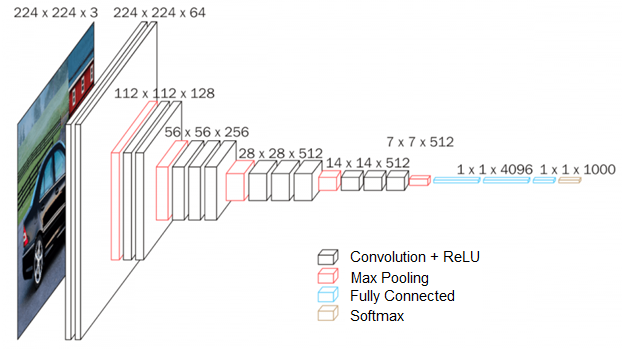
\includegraphics[width=0.6\linewidth]{images/vgg16_imagenet}
	\caption{Kiến trúc VGG16.}
	\label{fig:vgg16_imagenet}
\end{figure}
Đầu vào cho bất kỳ cấu hình mạng nào được coi là hình ảnh có kích thước cố định 224 x 224 với ba kênh R, G và B. Quá trình xử lý trước duy nhất được thực hiện là chuẩn hóa các giá trị RGB cho mỗi pixel. Điều này đạt được bằng cách trừ đi giá trị trung bình cho mỗi pixel.

Hình ảnh được chuyển qua ngăn xếp đầu tiên gồm 2 lớp tích chập có kích thước tiếp nhận rất nhỏ là 3 x 3, tiếp theo là kích hoạt ReLU. Mỗi lớp trong số hai lớp này chứa 64 bộ lọc. Stride được cố định ở 1 pixel và padding là 1 pixel. Cấu hình này bảo toàn độ phân giải không gian và kích thước của bản đồ kích hoạt đầu ra giống với kích thước hình ảnh đầu vào. Các bản đồ kích hoạt sau đó được chuyển qua tổng hợp tối đa không gian trên cửa sổ 2 x 2 pixel, với stride là 2 pixel. Điều này làm giảm một nửa kích thước của các lần kích hoạt. Do đó, kích thước của các kích hoạt ở cuối ngăn xếp đầu tiên là 112 x 112 x 64.

Các kích hoạt sau đó chảy qua ngăn xếp thứ hai tương tự, nhưng với 128 bộ lọc so với 64 bộ lọc trong ngăn xếp thứ nhất. Do đó, kích thước sau ngăn xếp thứ hai trở thành 56 x 56 x 128. Tiếp theo là ngăn xếp thứ ba với ba lớp chập và một lớp tổng hợp tối đa. Số lượng bộ lọc được áp dụng ở đây là 256, làm cho kích thước đầu ra của ngăn xếp là 28 x 28 x 256. Tiếp theo là hai ngăn xếp gồm ba lớp chập, với mỗi ngăn chứa 512 bộ lọc. Đầu ra ở cuối cả hai ngăn xếp này sẽ là 7 x 7 x 512.

Các chồng lớp chập trùng được theo sau bởi ba lớp được kết nối hoàn chỉnh với một lớp làm phẳng ở giữa. Hai lớp đầu tiên có 4.096 tế bào thần kinh mỗi lớp và lớp được kết nối đầy đủ cuối cùng đóng vai trò là lớp đầu ra và có 1.000 tế bào thần kinh tương ứng với 1.000 lớp có thể có cho tập dữ liệu ImageNet. Tiếp theo là lớp đầu ra là lớp kích hoạt Softmax được sử dụng để phân loại (Hình \ref{fig:vgg16_imagenet_detail}).

\begin{figure}[H]
	\centering
	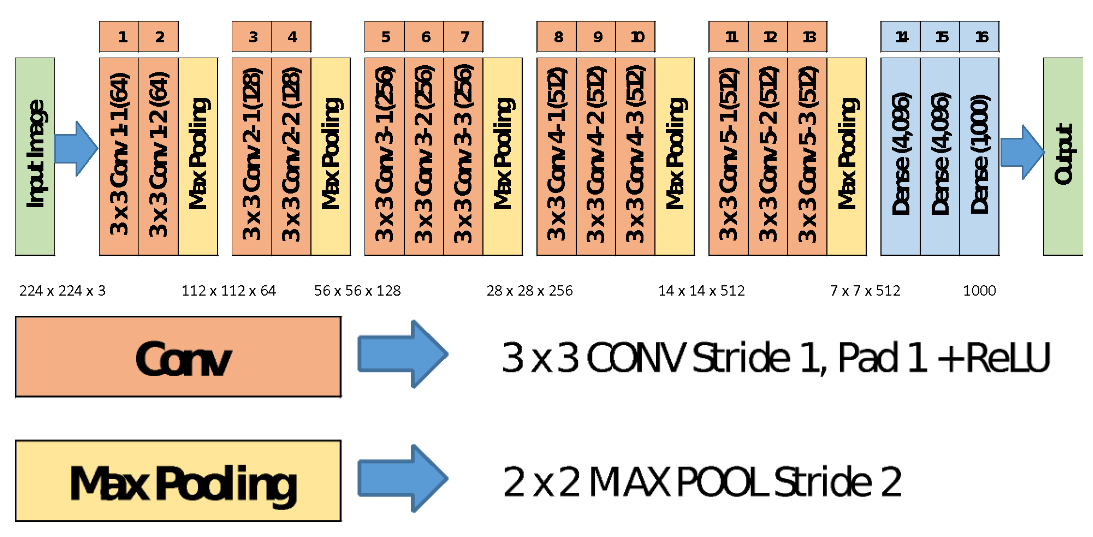
\includegraphics[width=1\linewidth]{images/vgg16_imagenet_detail}
	\caption{Kiến trúc VGG16.}
	\label{fig:vgg16_imagenet_detail}
\end{figure}

\subsection{Trường hợp sử dụng VGG16}
VGG16 khiến các nhà khoa học và nghiên cứu dữ liệu trên toàn thế giới quan tâm mặc dù sự ra đời của nhiều mô hình tính điểm mới và tốt hơn kể từ thời điểm VGG ban đầu được đề xuất. Dưới đây là một số trường hợp sử dụng mà bạn có thể thấy VGG16 được sử dụng thực tế:
\begin{enumerate}
	\item Nhận dạng hoặc phân loại hình ảnh - VGG16 có thể được sử dụng để chẩn đoán bệnh bằng hình ảnh y tế như X-quang hoặc MRI. Nó cũng có thể được sử dụng để nhận biết các biển báo đường phố từ một phương tiện đang di chuyển.
	\item Phát hiện và bản địa hóa hình ảnh - VGG16 có thể hoạt động thực sự tốt trong các trường hợp sử dụng phát hiện hình ảnh. Trên thực tế, nó đã là người chiến thắng trong thử thách phát hiện ImageNet vào năm 2014 (nơi nó kết thúc với vị trí á quân đầu tiên cho thử thách phân loại)
	\item Vectơ nhúng hình ảnh - Sau khi bật ra lớp đầu ra trên cùng, mô hình có thể được sử dụng để đào tạo để tạo vectơ nhúng hình ảnh có thể được sử dụng cho một vấn đề như xác minh khuôn mặt bằng cách sử dụng VGG16 bên trong mạng Siamese.
\end{enumerate}

\subsection{Áp dụng VGG16 vào bài toán của luận văn}
Có hai điểm khác biệt của tập dữ liệu ImageNet và tập dữ liệu \cite{dataset} được sử dụng trong bài toán của luận văn đó là:
\begin{enumerate}
	\item Kích thước ảnh đầu vào là 512x512 pixel thay vì 224x224 pixel và ảnh đầu vào là ảnh đa mức xám thay vì ảnh RGB.
	\item Chỉ có 2 lớp đầu ra: Có lao hay không có lao.
\end{enumerate}

Điều này dẫn tới 1 chút thay đổi nhỏ trong cấu hình của mô hình VGG16 cho bài toán này (hình \ref{fig:vgg16_luanvan}):
\begin{itemize}
	\item Ảnh đầu vào 512x512x1
	\item Vì chỉ có 2 lớp đầu ra nên neural đầu ra là 1, hàm kích hoạt là sigmoid. 
\end{itemize}
\begin{figure}[H]
	\centering
	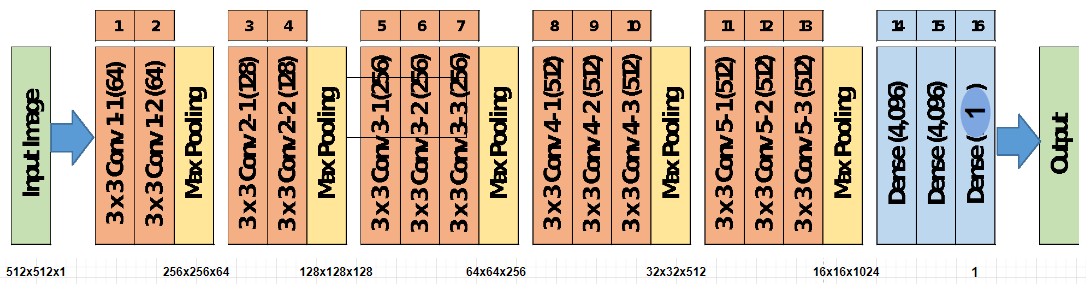
\includegraphics[width=1\linewidth]{images/vgg16_luanvan}
	\caption{Kiến trúc VGG16 cho bài toán của luận văn.}
	\label{fig:vgg16_luanvan}
\end{figure}

\subsection{Cài đặt mô hình}
\begin{lstlisting}[language=Python]
def make_vgg16_model(input_shape):
	inputs = keras.Input(shape=input_shape)
	x = data_augmentation(inputs)
	x = Rescaling(1.0 / 255)(x)
	#Block 1
	x = Conv2D(filters=start_step, kernel_size=(3, 3), padding='same', activation='relu', name='conv1_1')(x)
	x = Conv2D(filters=start_step, kernel_size=(3, 3), padding='same', activation='relu', name='conv1_2')(x)
	x = MaxPooling2D(pool_size=(2,2), strides=(2,2), name='max_pooling2d_1')(x)
	
	#Block 2
	x = Conv2D(filters=(start_step*2), kernel_size=(3, 3), padding='same', activation='relu', name='conv2_1')(x)
	x = Conv2D(filters=(start_step*2), kernel_size=(3, 3), padding='same', activation='relu', name='conv2_2')(x)
	x = MaxPooling2D(pool_size=(2,2), strides=(2,2), name='max_pooling2d_2')(x)
	
	#Block 3
	x = Conv2D(filters=(start_step*4), kernel_size=(3, 3), padding='same', activation='relu', name='conv3_1')(x)
	x = Conv2D(filters=(start_step*4), kernel_size=(3, 3), padding='same', activation='relu', name='conv3_2')(x)
	x = Conv2D(filters=(start_step*4), kernel_size=(3, 3), padding='same', activation='relu', name='conv3_3')(x)
	x = MaxPooling2D(pool_size=(2,2), strides=(2,2), name='max_pooling2d_3')(x)
	
	#Block 4
	x = Conv2D(filters=(start_step*8), kernel_size=(3, 3), padding='same', activation='relu', name='conv4_1')(x)
	x = Conv2D(filters=(start_step*8), kernel_size=(3, 3), padding='same', activation='relu', name='conv4_2')(x)
	x = Conv2D(filters=(start_step*8), kernel_size=(3, 3), padding='same', activation='relu', name='conv4_3')(x)
	x = MaxPooling2D(pool_size=(2,2), strides=(2,2), name='max_pooling2d_4')(x)
	
	#Block 5
	x = Conv2D(filters=(start_step*8), kernel_size=(3, 3), padding='same', activation='relu', name='conv5_1')(x)
	x = Conv2D(filters=(start_step*8), kernel_size=(3, 3), padding='same', activation='relu', name='conv5_2')(x)
	x = Conv2D(filters=(start_step*8), kernel_size=(3, 3), padding='same', activation='relu', name='conv5_3')(x)
	x = MaxPooling2D(pool_size=(2,2), strides=(2,2), name='max_pooling2d_5')(x)
	
	#Flatten and FC
	x = Flatten(name='flatten')(x)
	x = Dense((start_step*8), activation='relu', name='fc_1')(x)
	x = Dropout(0.5, name='dropout_1')(x)
	x = Dense((start_step*4), activation='relu', name='fc_2')(x)
	x = Dropout(0.5, name='dropout_2')(x)
	outputs = Dense(1, activation='sigmoid', name='output')(x)
	return keras.Model(inputs,outputs)			
\end{lstlisting}

	 
	 

\setcounter{chapter}{2}
\setcounter{section}{1}
\chapter{\tenchuongiii}
\section{Phân tích yêu cầu bài toán}
Như đã nói tại Chương 1, bài toán phân loại hình ảnh của luận văn là một trong những nhiệm vụ phổ biến trong Computer Vision. Mục tiêu chính của bài toán này đó chính là phân loại một hình ảnh đầu vào (input) thành một nhãn (label) đầu ra (output).  

Với bài toán phân loại ảnh của luận văn, ta có tập dữ liệu ảnh chụp x-quang phổi đã được gán nhãn làm hình ảnh đầu vào (input). Hình ảnh có định dạng PNG như hình \ref{fig:normalimg}.

Tập dữ liệu trên được một nhóm các nhà nghiên cứu từ Đại học Qatar, Doha, và Đại học Dhaka, Bangladesh cùng với các cộng tác viên của họ từ Malaysia phối hợp với các bác sĩ từ Hamad Medical Corporation và Bangladesh đã tạo ra một cơ sở dữ liệu về hình ảnh X-quang phổi cho người có lao cùng với hình ảnh người không có lao \cite{dataset}. Dữ liệu trên được cung cấp miễn phí tại \href{https://www.kaggle.com/datasets/tawsifurrahman/tuberculosis-tb-chest-xray-dataset}{https://www.kaggle.com/datasets/tawsifurrahman/tuberculosis-tb-chest-xray-dataset}. Thông tin cụ thể về tập dữ liệu như sau:
\begin{itemize}
	\item Tổng số 4200 ảnh đã được phân loại thành hai thư mục Normal (bình thường) và Tuberculosis (có lao).
	\item Số ảnh người mắc lao: 700 ảnh.
	\item Số ảnh người không mắc lao: 3500 ảnh.
	\item Kích thước ảnh: 512 x 512 (pixel)
	\item Định dạng ảnh: PNG.
	\item Tập tin Normal.metadata.xlsx tổng hợp thông tin về các file ảnh của người không mắc lao.
	\item Tập tin Tuberculosis.metadata.xlsx tổng hợp thông tin về các file ảnh của người mắc lao.
\end{itemize}

Mục tiêu mong muốn của bài toán là việc có thể dự đoán về khả năng ảnh x-quang phổi được đưa vào là của người có lao hay không, đây là nhãn (label) đầu ra (output) mong muốn, dựa vào nhãn đầu ra này ta sẽ kết luận xem người có ảnh chụp x-quang đó có bị lao hay tổn thương phổi không. Để thực hiện được mục tiêu trên, ta cần thực hiện hai pha:
\begin{itemize}
	\item \textbf{Học:} Lặp lại nhiều lần việc lần lượt đưa tất cả ảnh đầu vào để huấn luyện mô hình, trích chọn ra các đặc trưng của ảnh rồi lưu lại. Quá trình này nên dừng lại khi độ chính xác đạt mức tối thiểu mà ta đặt ra hoặc độ chính xác tăng lên không đáng kể sau một số lượt huấn luyện nhất định. 
	\item \textbf{Phân loại:} Dùng các đặc trưng mà mô hình thu được tại pha Học, đưa ảnh chụp x-quang đầu vào để tiến hành so sánh với các đặc trưng đó, kết thúc quá trình bằng một giá trị dự đoán khả năng mắc lao của người có ảnh x-quang được đưa vào.
\end{itemize}

Để đảm bảo tính chính xác, khách quan cho khả năng dự đoán của mô hình đã đào tạo, ta cần tách dữ liệu cho hai pha này phải khác nhau. Ta có thể tách riêng 100 ảnh trong tập dữ liệu bao gồm cả ảnh x-quang của người có lao và không có lao là một tập dữ liệu mới gọi là dữ liệu xác thực để sử dụng cho pha Phân loại. Còn lại 4100 ảnh x-quang của tập dữ liệu gốc ta gọi là dữ liệu huấn luyện và sử dụng cho pha Học.

\section{Phân tích lựa chọn công cụ}
\subsection{Lựa chọn mô hình đã hệ thống hóa}
Tại công bố của Karen Simonyan và Andrew Zisserman \cite{vgg16}, các tác giả có thông tin mạng VGG có số lượng tham số khổng lồ từ 133 - 144 triệu. Với hệ thống được hỗ trợ là bốn NVIDIA Titan Black GPUs, việc đào tạo một mô hình đơn chiếm tới 2-3 tuần tùy thuộc vào cấu trúc. Chính vì vấn đề thời gian và nguồn tài nguyên nghiên cứu không thể đáp ứng nên chương trình thử nghiệm sẽ không áp dụng mô hình VGG.
 
Tham khảo kết quả nghiên cứu được công bố của Gao Huang \cite{densenet} được thông tin tại hình \ref{fig:selected_model} về so sánh tỷ lệ lỗi trên tập dữ liệu CIFAR và SVHN của các mô hình CNN, đặc biệt là mô hình ResNet và các biến thể của nó, ta dễ dàng nhận ra DenseNet có tỉ lể lỗi thấp hơn so với các mô hình ResNet, số lượng tham số cũng có ít hơn ResNet. Từ đây có thể nhận thấy rõ nên áp dụng mô hình DenseNet.
\begin{figure}[H]
	\centering
	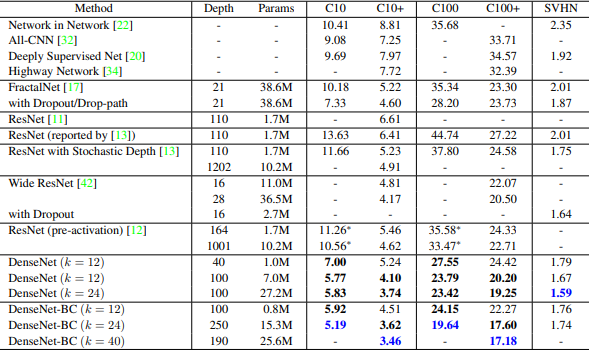
\includegraphics[width=1\linewidth]{images/selected_model}
	\caption{Tỉ lể lỗi trên tập dữ liệu CIFAR và SVHN của các mô hình CNN.}
	\label{fig:selected_model}
\end{figure}

Chính vì những cơ sở trên, học viên quyết định sử dụng mô hình DenseNet cho phần mềm thử nghiệm của luận văn.

\subsection{Phân tích mô hình hệ thống}
Hệ thống chương trình thử nghiệm Phần mềm chuẩn đoán bệnh lao được thiết kế theo kiến trúc Client/Server năm tầng (hình \ref{fig:client_server_ntang}), trong đó:
\begin{itemize}
	\item {\bf Tầng thứ nhất} là tầng giao diện người phân loại, cụ thể là ứng dụng client trên trình duyệt, quản lý tương tác người phân loại với ứng dụng như chọn ảnh gửi lên server… và hiển thị kết quả phân loại do server gửi về.
	\item {\bf Tầng thứ hai} là tầng server quản lý cấu hình hệ thống, ví dụ cấu hình giao thức gửi/nhận dữ liệu với client, cụ thể giao thức được sử dụng trong hệ thống là giao thức HTTP.
	\item {\bf Tầng thứ ba} là tầng server thực hiện logic xử lý các yêu cầu từ client, như	quản lý và phân phối các luồng xử lý độc lập, đảm bảo hiệu năng và chất lượng tính toán phân loại cho nhiều client trong cùng một thời điểm.
	\item {\bf Tầng thứ tư} là tầng đảm nhiệm xây dựng, tinh chỉnh và quản lý các phiên	bản mô hình phân loại cho hệ thống, với bộ ảnh huấn luyện được lấy từ tầng quản lý dữ liệu bên dưới.
	\item {\bf Tầng cuối cùng} là tầng quản lý dữ liệu, bao gồm CSDL ảnh phục vụ cho việc huấn luyện mô hình, CSDL ảnh đã xử lý từ các client nhằm mục đích bổ sung sự	đa dạng của CSDL ảnh và cải thiện độ chính xác của mô hình phân loại. Các bộ ảnh trên được lưu tách biệt để thuận tiện cho việc quản lý và đánh giá độ chính xác của các
	phiên bản mô hình huấn luyện cũng như mức độ ảnh hưởng của bộ ảnh huấn luyện lên chất lượng mô hình.
\end{itemize}
\begin{figure}[H]
	\centering
	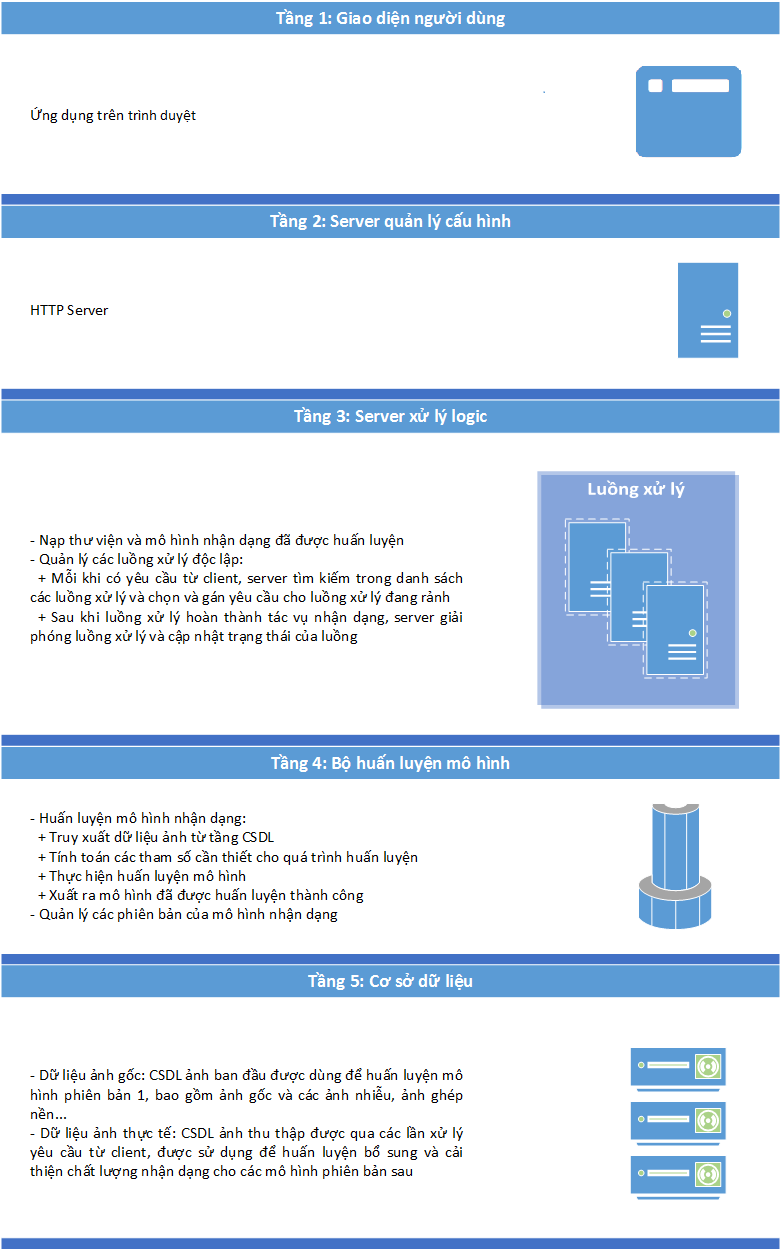
\includegraphics[width=1\linewidth]{images/client_server_ntang}
	\caption{Kiến trúc Client/Server năm tầng.}
	\label{fig:client_server_ntang}
\end{figure}

Luồng hoạt động chính của hệ thống được thể hiện trong hình \ref{fig:app_sequence}, trong đó các bước thực hiện của server và client từ lúc khởi động ban đầu tới lúc kết thúc như sau:
\begin{itemize}
	\item Client (ứng dụng trên trình duyệt)
	\begin{enumerate}
		\item Người phân loại khởi động ứng dụng/website.
		\item Người phân loại thực hiện chọn ảnh chụp x-quang trước đó được lưu trong máy tính để gửi.
		\item Ảnh chụp được mã hóa, nén lại và gửi tới máy chủ.
		\item Ứng dụng đợi nhận kết quả phân loại từ máy chủ gửi về và hiển thị cho người phân loại
	\end{enumerate}
	\item Chương trình Server
	\begin{enumerate}
		\item Chương trình được khởi động và nạp các thư viện cần thiết.
		\item Chương trình nạp mô hình phân loại đã được huấn luyện trước đó.
		\item Giao thức gửi, nhận dữ liệu giữa ứng dụng phía client và chương trình server được cấu hình.
		\item Một loại các luồng xử lý được khởi tạo, đặt trạng thái ban đầu là trạng thái sẵn sàng.
		\item Khi có ứng dụng client kết nối tới, chương trình kiểm tra trong danh sách các luồng xử lý và chọn một luồng đang ở trạng thái sẵn sàng để nhận và tính toán dữ liệu do client gửi tới.
		\item Trong luồng xử lý:
		\begin{itemize}
			\item Bắt đầu quá trình tính toán phân loại, cờ trạng thái là “bận”.
			\item Thực hiện giải nén dữ liệu thành dữ liệu ảnh gốc.
			\item Sử dụng mô hình đã nạp để phân loại ảnh.
			\item Trả kết quả phân loại về cho ứng dụng client.
			\item Kết thúc quá trình tính toán.
		\end{itemize}
		\item Khi luồng xử lý đã hoàn thành quá trình tính toán phân loại, chương trình giải phóng luồng xử lý bằng cách cập nhật lại trạng thái hiện tại của luồng.
	\end{enumerate}
\end{itemize}
\begin{figure}[H]
	\centering
	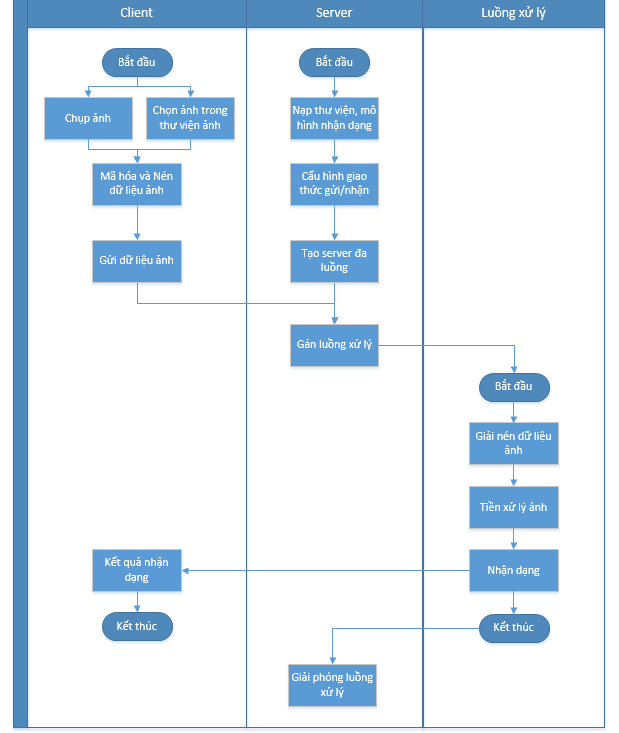
\includegraphics[width=1\linewidth]{images/app_sequence}
	\caption{Luồng hoạt động chính của hệ thống.}
	\label{fig:app_sequence}
\end{figure}

\section{Một số kết quả chương trình}
\subsection{Một số giao diện và chức năng chính chính của chương trình}
\subsection{Giao diện đăng nhập hệ thống}
Giao diện đăng nhập hệ thống cung cấp lớp bảo vệ cơ bản cùng khả năng định danh người dùng, từ đó đưa ra nhưng ngữ cảnh thực đơn phù hợp.
\begin{figure}[H]
	\centering
	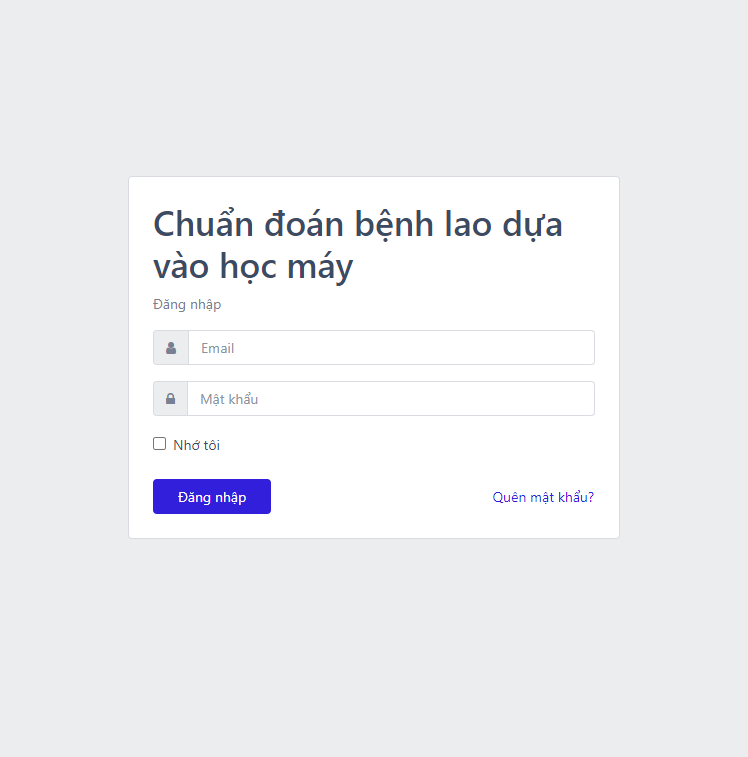
\includegraphics[width=1\linewidth]{images/giaodien_dangnhap}
	\caption{Giao diện đăng nhập hệ thống.}
	\label{fig:giaodien_dangnhap}
\end{figure}

\subsubsection{Giao diện cập nhật mô hình}
Tại đây, quản trị viên có thể thay đổi mô hình được sử dụng trong hệ thống. Mô hình này là được tạo ra ở pha Học. Mô hình mới được tải lên server, lưu trữ lại và ghi lại thông tin về đường dẫn để hệ thống có thể gọi được khi cần thiết.
\begin{figure}[H]
	\centering
	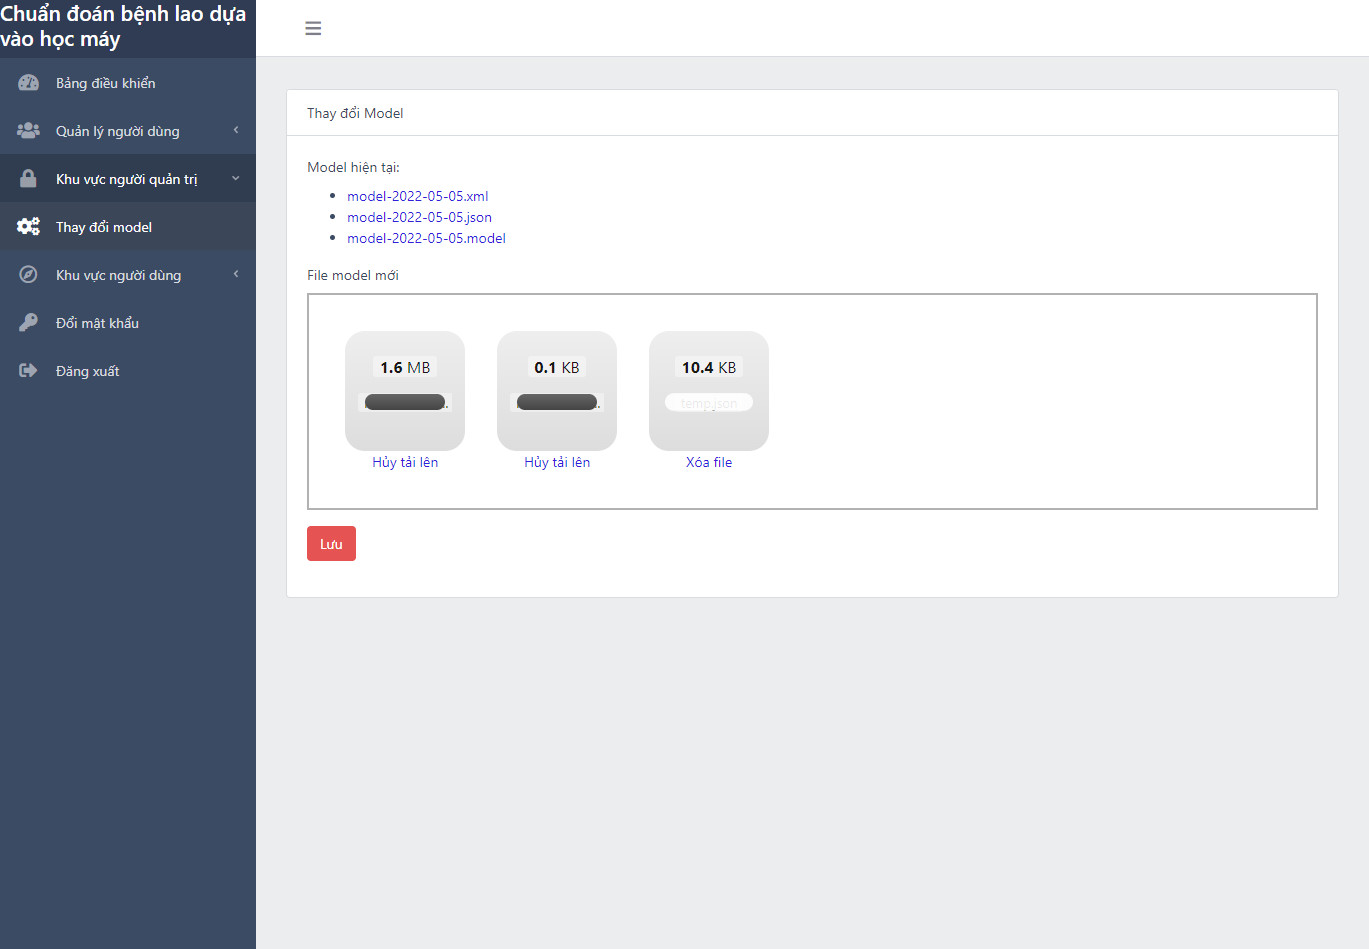
\includegraphics[width=1\linewidth]{images/quantri_doi_model}
	\caption{Giao diện cập nhật mô hình được sử dụng của hệ thống.}
	\label{fig:quantri_doi_model}
\end{figure}

\subsubsection{Giao diện danh sách các dự đoán}
Giao diện này tập trung thông tin của tất cả các dự đoán đã được thực hiện và lưu lại của hệ thống. Hệ thống sẽ hiện thị tất cả các dự đoán đối với người quản trị, và với tài khoản người dùng, hệ thống chỉ hiển thị những dự đoán thuộc về người dùng.
\begin{figure}[H]
	\centering
	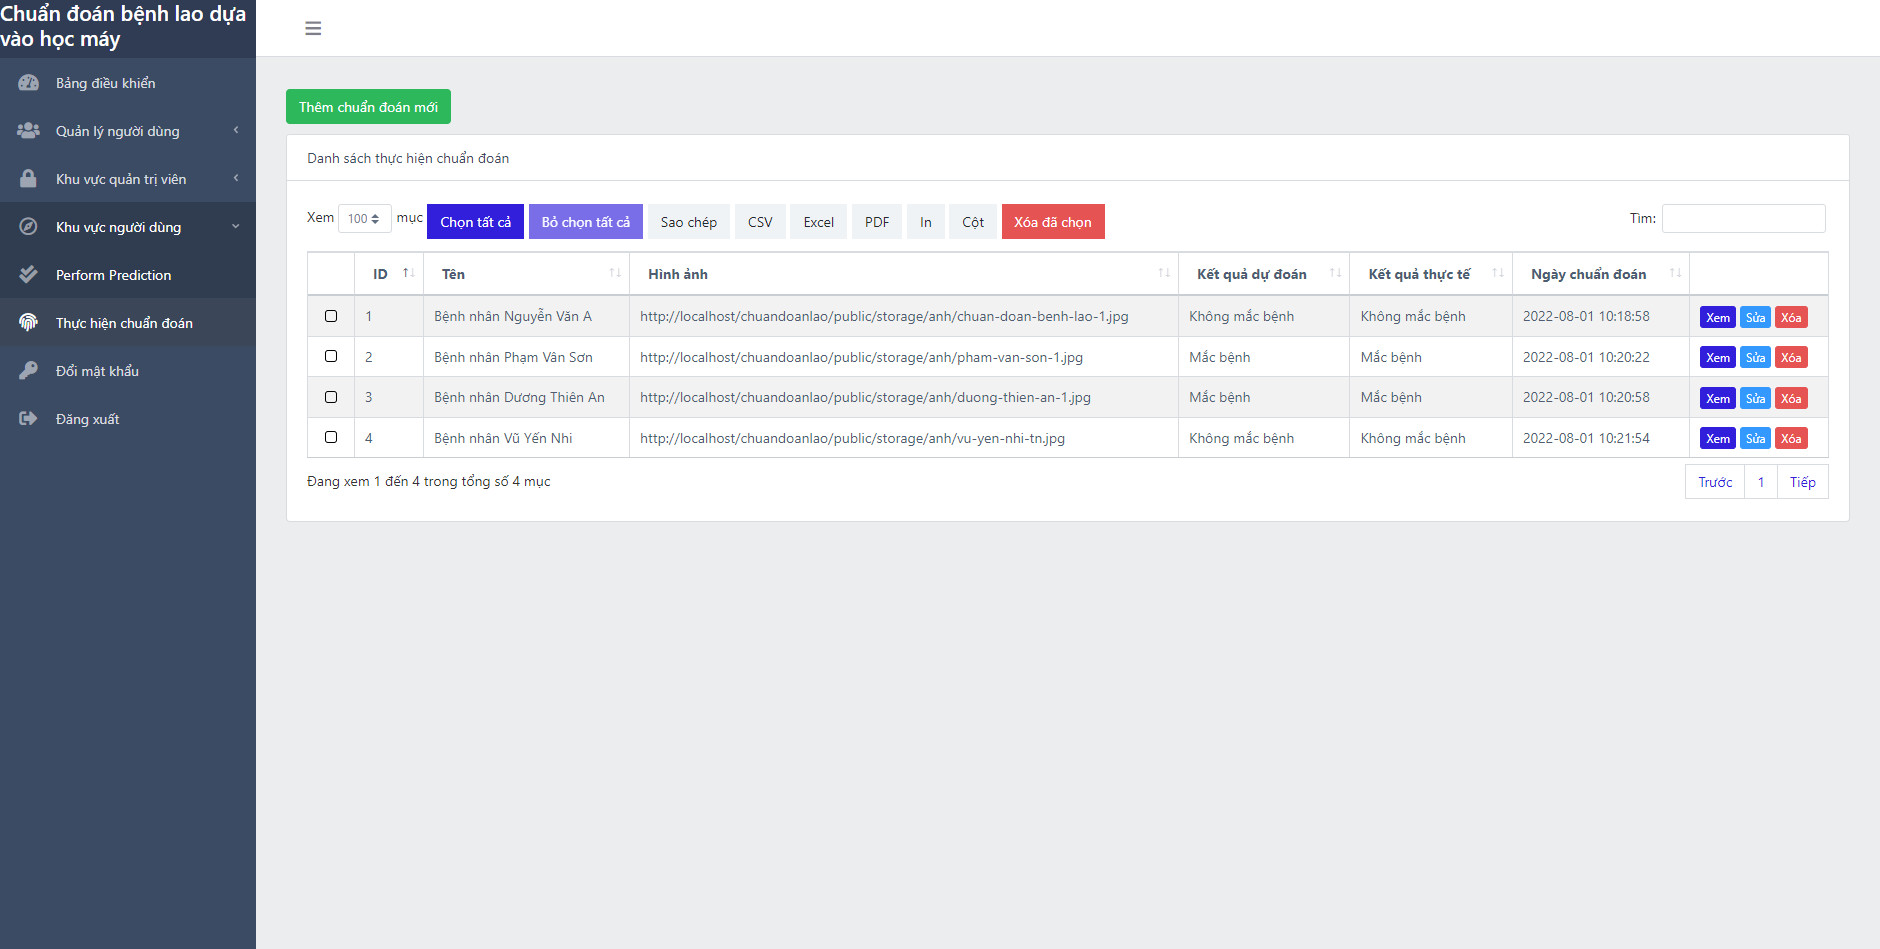
\includegraphics[width=0.95\linewidth]{images/user_danh_sach}
	\caption{Giao diện danh sách các dự đoán của hệ thống.}
	\label{fig:user_danh_sach}
\end{figure}

\subsection{Giao diện thực hiện dự đoán}
Người dùng upload ảnh chụp x-quang đã chuyển đổi định dạng PNG với kích thước 512x512 tại đây và nhận về kết quả dự đoán.
\begin{figure}[H]
	\centering
	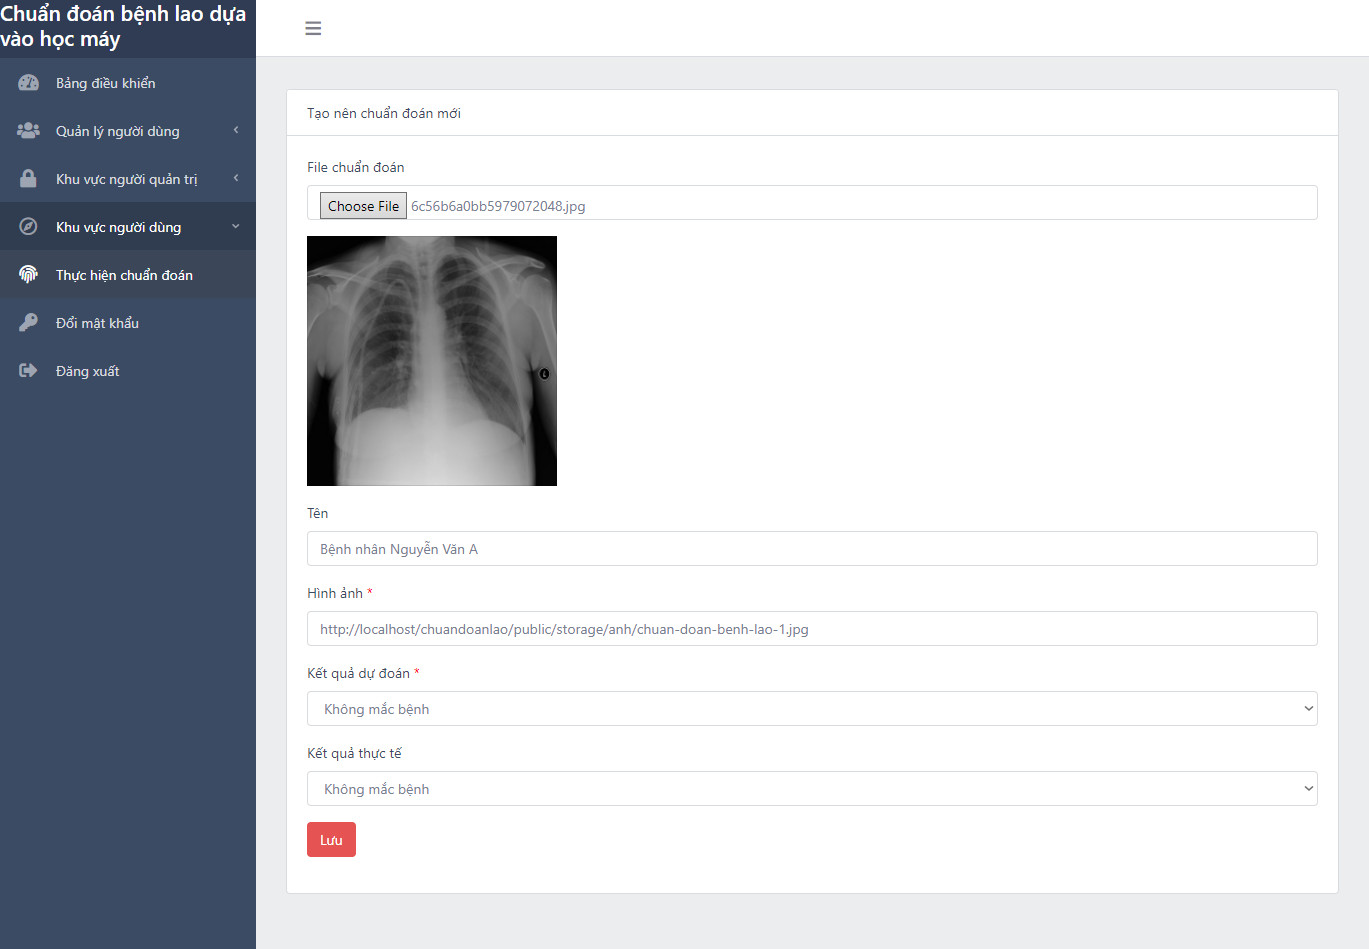
\includegraphics[width=0.95\linewidth]{images/user_du_doan_chi_tiet}
	\caption{Giao diện thực hiện phân loại của hệ thống.}
	\label{fig:user_danh_sach}
\end{figure}

\subsection{Một số ca phân loại được thực hiện bởi chương trình}
Thực hiện kiểm thử việc phân loại của hệ thống với 100 ảnh x-quang được tách riêng biệt khỏi quá trình trainning, ta có được kết quả rất khả quan.
\begin{figure}[H]
	\centering
	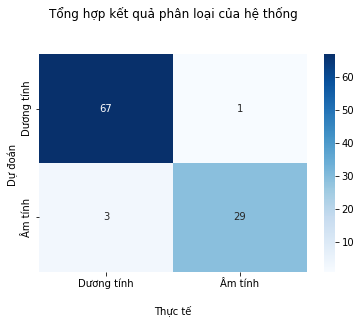
\includegraphics[width=0.66\linewidth]{images/result_backtest}
	\caption{Tổng hợp các ca phân loại của hệ thống.}
	\label{fig:result_backtest}
\end{figure}
Bài toán của luận văn chỉ có hai lớp để phân loại nên phương pháp thích hợp nhất để đánh giá là True/False Positive/Negative. Ta định nghĩa lớp dữ liệu quan trọng hơn cần được xác định đúng là lớp Positive (P-dương tính), lớp còn lại được gọi là Negative (N-âm tính). Ta định nghĩa True Positive (TP), False Positive (FP), True Negative (TN), False Negative (FN) dựa trên confusion matrix chưa chuẩn hoá. 

Bằng phương pháp trên, ta có kết quả tổng hợp tại hình \ref{fig:result_backtest}, tỉ lệ dự đoán chính xác là 96\%, tỉ lệ báo động nhầm (False Alarm Rate) là 1\% và tỉ lệ bỏ sót (Miss Detection Rate) là 3\%.  

\chapter*{\begin{center}Kết luận\end{center}}
\addcontentsline{toc}{chapter}{Kết luận}
Phân loại ảnh số là một lĩnh vực nghiên cứu hấp dẫn vì có thể áp dụng trong rất nhiều bài toán thực tế. Đây cũng là một bài toán phức tạp nhưng không quá khó để giải quyết nếu ta biết ứng dụng các thành tựu nghiên cứu trong các lĩnh vực như xử lý ảnh số, trí tuệ nhân tạo… Trong đó, việc ứng dụng thành quả của Deep learning mà trong đó đặc biệt là các mô hình của mạng CNN cho ta các kết quả thực sự ấn tượng.

\section*{Kết quả đã đạt được}
Sau một thời gian tìm hiểu nghiên cứu, luận văn đã trình bày được các vấn đề sau:
\begin{itemize}
	\item Trình bày khái quát về CNN và bài toán chẩn đoán bệnh lao
	\item Hệ thống hóa một số mô hình học sâu hỗ trợ chẩn đoán
	\item Cài đặt thử nghiệm một trong các mô hình đã được hệ thống hóa
\end{itemize}

\section*{Hướng hoàn thiện và phát triển tiếp theo:}
Chương trình tuy đã đảm bảo được những chức năng chính yếu nhất của luận văn, nhưng để áp dụng vào thực tế thì vẫn chưa thể được. Lý do chính cho việc này là do sự khác biệt giữa nguồn ảnh đầu vào. Như đã trình bày ở Chương 3, nguồn ảnh đầu vào của bài toán luận văn là ảnh định dạng PNG, tuy nhiên, thực tế nguồn ảnh x-quang y tế được chụp qua các thiết bị thu nhận ảnh y tế (CT, MRI...) hầu hết lại ở định dạng DICOM. Việc không đồng nhất về định dạng ảnh khiến cho chương trình hiện nay chưa thể đưa vào sử dụng trong thực tế.

Một vấn đề khác khi nghiên cứu bài toán của luận văn với bộ dữ liệu do Tawsifur Rahman và cộng sự \cite{dataset} cung cấp là chất lượng ảnh đầu vào không đồng đều. Hầu hết ảnh trong bộ dữ liệu đều có chất lượng tốt, sắc nét, rõ ràng. Nhưng cũng có một vài ảnh mờ, không thực sự rõ nét. Ảnh chất lưởng kém hơn ít nhiều cũng sẽ ảnh hưởng đến độ chính xác của chương trình. Việc nâng cao chất lượng ảnh đầu vào cho chương trình nói riêng và cả lĩnh vực Thị giác Máy - Computer Vision - nói chung là vấn đề rất quan trọng. 

Từ những vấn đề nêu trên, học viên đề xuất hướng phát triển tiếp theo là hoàn thiện thêm các chức năng liên quan đến nâng cao chất lượng ảnh đầu vào, chức năng kết nối với thiết bị thu nhận ảnh y tế (CT, MRI...) để hoàn thiện chương trình có thể ứng dụng vào thực tiễn.
\addcontentsline{toc}{chapter}{Tài liệu tham khảo}
\begin{thebibliography}{99}
	\bibitem{gtcreport} WHO {\it Global tuberculosis report 2020}, báo cáo tại \href{https://www.who.int/publications/i/item/9789240013131}{ https://www.who.int/publications/i/item/9789240013131}, 2020
	
	\bibitem{bytchuandoanlao} Bộ Y tế {\it Chuẩn đoán bệnh lao}, \href{https://healthvietnam.vn/thu-vien/tai-lieu-tieng-viet/ho-hap/chan-doan-benh-lao}{https://healthvietnam.vn/thu-vien/tai-lieu-tieng-viet/ho-hap/chan-doan-benh-lao}, 2015
	
	%\bibitem{ntt8b3} Nguyễn Thanh Tuấn {\it Neural network}, https://nttuan8.com/bai-3-neural-network, 2019
	
	\bibitem{ntt} Nguyễn Thanh Tuấn {\it Deep learning cơ bản (Chưa xuất bản)}, \href{https://drive.google.com/file/d/1lNjzISABdoc7SRq8tg-xkCRRZRABPCKi/view}{https://drive.google.com/file/d/1lNjzISABdoc7SRq8tg-xkCRRZRABPCKi/view}, 2019
	
	\bibitem{densenetlagi} Võ Thị Một, Võ Duy Nguyên, Nguyễn Tấn Trần Minh Khang {\it Trích chọn đặc trưng và phân loại ảnh x-quang phổi}, TNU Journal of Science and Technology 226(07): 182 - 189 {\href{http://jst.tnu.edu.vn/jst/article/viewFile/3974/pdf}{PDF}}, 2021
	
	\bibitem{dataset} Tawsifur Rahman, Amith Khandakar, Muhammad A. Kadir, Khandaker R. Islam, Khandaker F. Islam, Zaid B. Mahbub, Mohamed Arselene Ayari, Muhammad E. H. Chowdhury {\it Reliable Tuberculosis Detection using Chest X-ray with Deep Learning, Segmentation and Visualization}, IEEE Access - Vol. 8, 2020
	
	\bibitem{cnnhumanbrain} Grace W. Lindsay {\it Convolutional Neural Networks as a Model of the Visual System: Past, Present, and Future}, arXiv - Cornell University (\href{https://arxiv.org/ftp/arxiv/papers/2001/2001.07092.pdf}{PDF}), 2001
	
	\bibitem{vgg16} Karen Simonyan, Andrew Zisserman {\it Very deep convolutional networks for large-scale image recognition}, ICLR 2015 (\href{https://arxiv.org/pdf/1409.1556.pdf}{PDF}), 2015
	
	\bibitem{densenet} Gao Huang, Zhuang Liu, Laurens van der Maaten, Kilian Q. Weinberger {\it Densely Connected Convolutional Networks}, arXiv:1608.06993 (\href{https://arxiv.org/pdf/1608.06993.pdf}{PDF}), 2016 
	  
\end{thebibliography}


\end{document}


